\section{Overview}
The main aspects of the design are:
\begin{itemize}
    \item \textbf{Microservices}. The system architecture is \ac{SOA}. In particular it follows the Microservices architecture.
    \item \textbf{Event-Based Architecture}. The service to service communication is thought with an event based fashion. Each component is either a producer or consumer of an event, for example when a tournament is a created one module will advertise it and another module will see the event and notify users.
    \item \textbf{Restful API}. The user communicates with the system by using REST interfaces provided by the front end services. 
\end{itemize}
The system also exploits a third party email service to communicate notification to the user and uses GitHub APIs for the management of battle repository.
The following diagram represents how the system interacts with the world.
\begin{figure}[H]
    \centering
    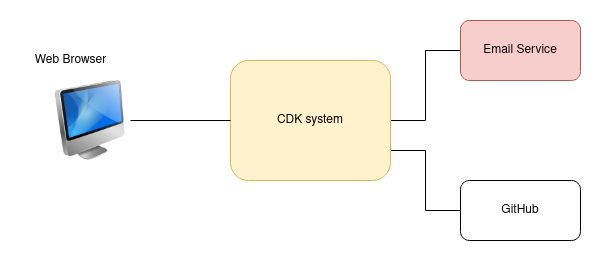
\includegraphics[width=1\linewidth]{misc/overviewDiagram.png}
    \caption{High Level View Diagram}
    \label{fig:enter-label}
\end{figure}

\newpage

\section{Component View}

The component diagram shows all the identified components and their interactions. We provide two different diagrams: 
\begin{itemize}
    \item In the first one we show how the various microservices interact with each other
    \item In the second one we show how the microservices interact with the external world.
\end{itemize}

After the diagrams a brief description of all the components will follow.

\subsection{Component Diagram}

\subsubsection{System Interaction}

\begin{figure}[H]
    \centering
    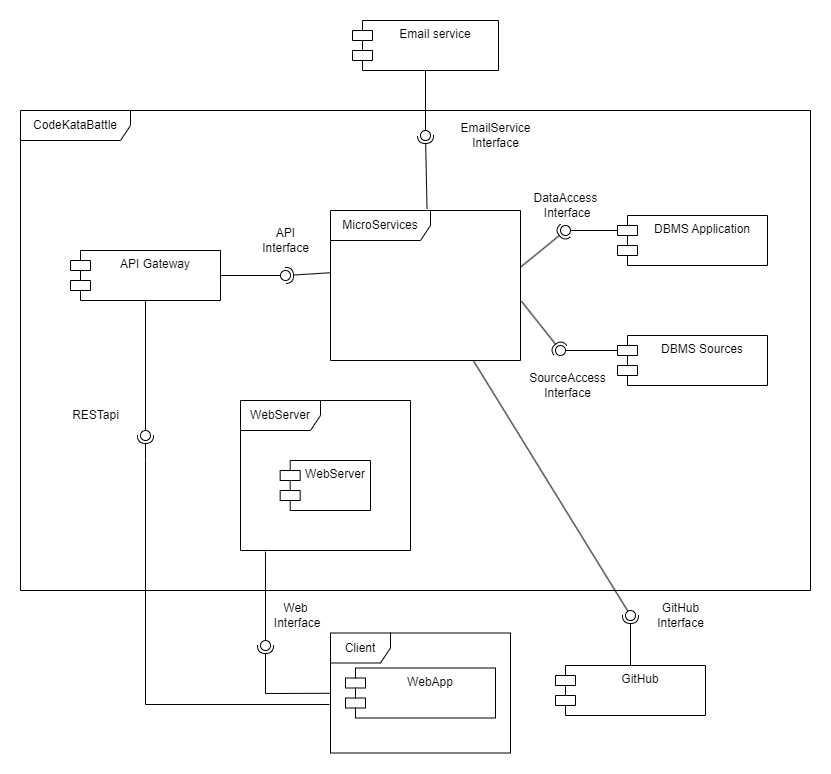
\includegraphics[width=1\linewidth]{misc//Images/Component.png}
    \caption{\ac{CKB} component diagram}
    \label{fig:enter-label}
\end{figure}

\subsubsection{Microservices Interaction}

\begin{figure}[H]
    \centering
    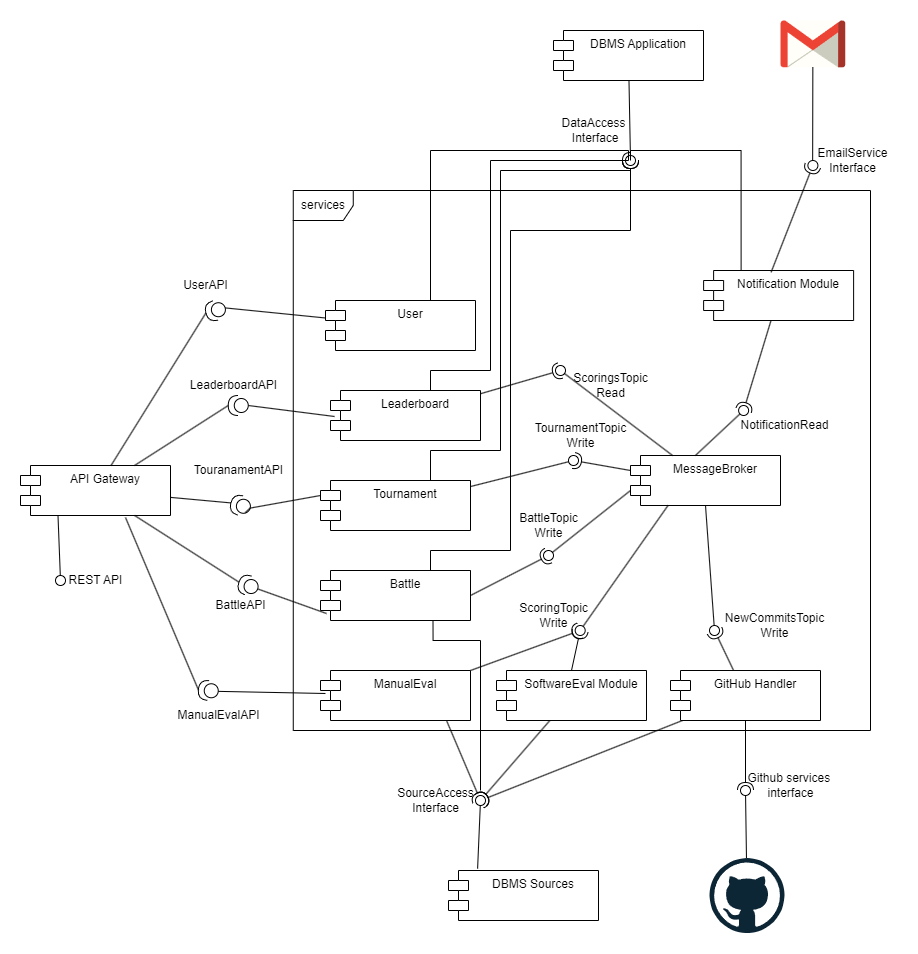
\includegraphics[width=1\linewidth]{misc//Images/microservicesComponentDiagram.png}
    \caption{\ac{CKB} Microservices Interactions}
    \label{fig:enter-label}
\end{figure}

\subsection{Components description}

The components are: 
\begin{itemize}
    \item GitHub handler :    Interfaces with GitHub APIs in order to: 
    \begin{itemize}
        \item create a Repository for a Battle after the subscription deadline
        \item retrieve the source code from a group after any commit and store it on a DataBase so that it can be automatically evaluated and then manually evaluated if needed during the consolidation phase
    \end{itemize}
\item Message broker :  It is the component tasked with dealing with messages from other services to enstablish the event based comunication between services. It keeps message queues for the various topics which some services produce and other are subscribe to
\item Email service :   Its is a third party service, used to send users various notifications.
\item User service: this component handles all the login and registration logic but not the authentication one.
\item API gateway : It handles client access to the various system services, it also handles the authorization aspects of the services use, to ensure system security.
\item Web server : It interfaces with the client browser and responds to its requests with the needed web pages(html+css+js).
\item WebApp : The part of the application that runs on the client browser. It is made of a set of web pages which are able to make requests to the web server and the services the system provides.
\item Github : It is the third party application that handles the battle repositories. 
\begin{itemize}
    \item The student users use its services outside the \ac{CKB} scope to fork a \ac{CK} assignement and work on its solution.
    \item The \ac{CKB} system interfaces with some Github services in order to create the repository and retrieve the solutions committed by students for evaluation.
\end{itemize}
\item DBMS (Application) : It is the DBMS that provides access to the database containting all the information about users, tournaments, battles and the scoring.
\item DBMS (Sources) : The DBMS for the database that keeps the source code related to any groups in any battles. This database is separated from the other in order to :
\begin{itemize}
    \item Optimize its performance , since the dimension of its records can be possibly way bigger.
    \item Have better control on the source codes to be stored, since they will run inside the \ac{CKB} system for evaluation, making it a security concern.
\end{itemize}
\item Tournament Service: The tournament service handles all aspects of a tournament, from the creation to the joining of students.
\item Battle Service: The battle service handles all aspects of a battle,  from the creation to the joining of students.
\item Notification Service: The notification Service handles all the user notifications. Students and Educators are gonna get email notification from this service whenever: a new tournament is created, a new battle is created, a final rank for a battle is available and a final battle for a tournament is available.
\item Leaderboard Service: The service handles all kinds of leaderboards present in the system. It exchanges messages with ManualEval and SoftwareEval and through those it updates the leaderboards of battles and tournaments inside the Application DBMS.
\item ManualEval Service: The component handles the consolidation stage of a battle(if it was required). It gives access to a group's sources in order to add a new score for the battle the group is participating.
\item SoftwareEval Service: The component handles the automatic scoring of new commits to the group's repository. Whenever a student commits to the repository GitHub sends a notification to the GithubHandler service which downloads the sources and signals to this component the neediness of an Evaluation
\end{itemize}
\newpage
\section{Deployment view}

The following deployment diagram shows how all the components are distributed and how they interact with each other.

\begin{figure}[H]
    \centering
    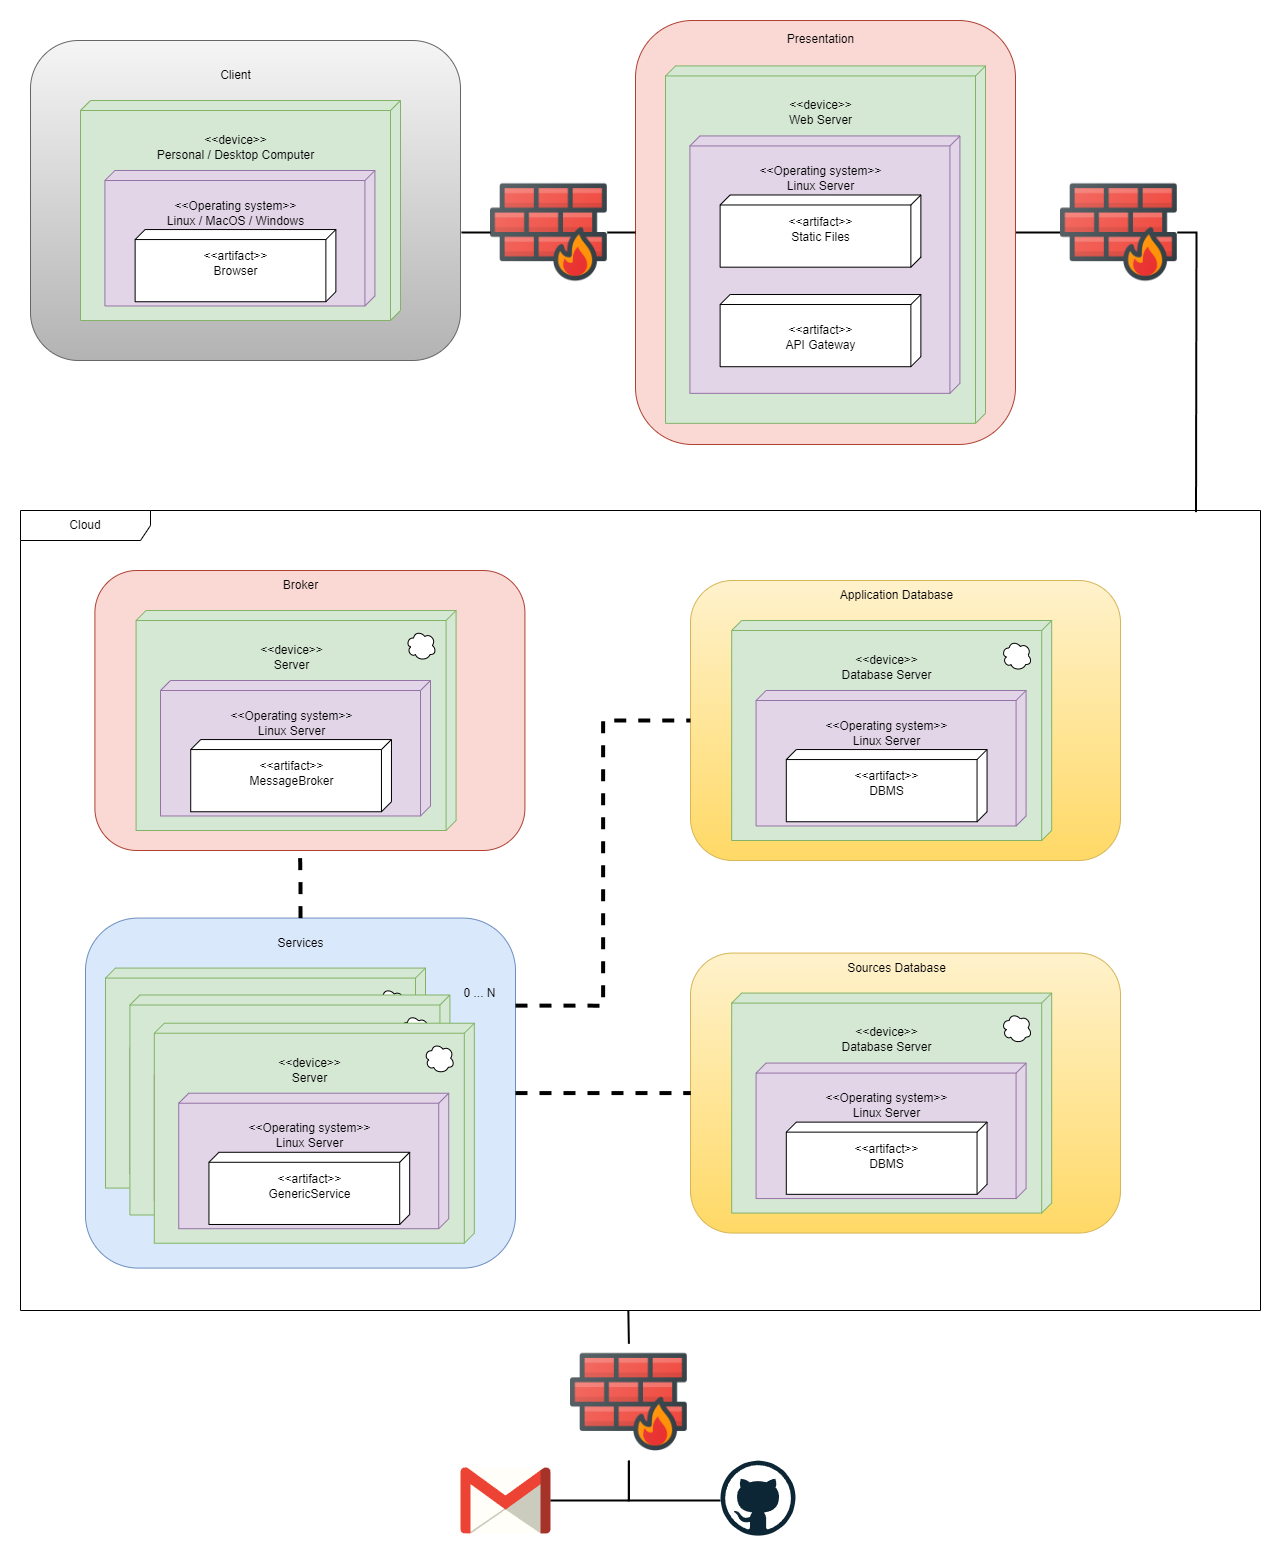
\includegraphics[width=1\linewidth]{misc//Images/Deployment.png}
    \caption{\ac{CKB} Deployement diagram}
    \label{fig:enter-label}
\end{figure}

\section{Runtime view}

Here we present the dynamics of our system through the use of sequence diagrams. All the interaction that use REST APIs start with the client request to an API that may contain a number of parameters, which are listed in the interface description of the API in the apposite document section, and end with either a positive response, eventually containing requested data and/or hyperlink for contextual page navigation (following REST's HATEOAS principle), or a negative response in case of any error.
For reading simplicity only positive responses are shown in the diagrams, as any other error response sent to the client always results in an error alert in the client application page.
In the interactions where the notification service is involved an email containing a message for the users is sent. The message content and destination is in the diagram description.
In some complex diagrams where the message broker is involved, a more specific description of its interaction with the other services is provided.

\subsection{Sign Up}

After the user has signed up, the positive REST response contains the hypertext to redirect the client to the tournament's main page.

\begin{figure}[H]
    \centering
    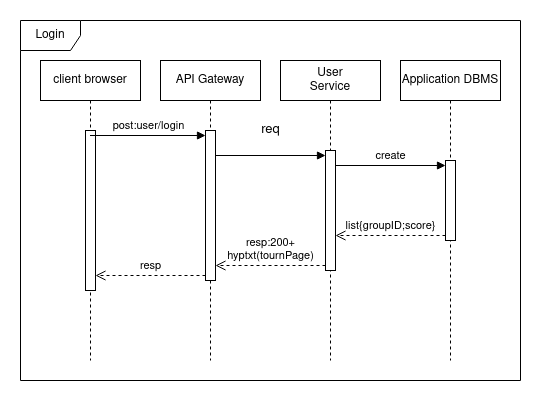
\includegraphics[width=1\linewidth]{misc//Images//UC/UC2.png}
    \caption{Sign up sequence diagram}
    \label{fig:enter-label}
\end{figure}
\newpage
\subsection{Sign In}

After the user has signed in, the positive rest response contains the hypertext to redirect the client to the tournaments main page.

\begin{figure}[H]
    \centering
    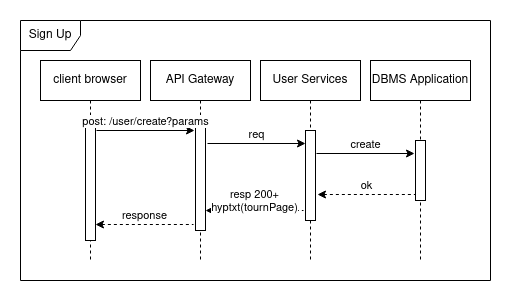
\includegraphics[width=1\linewidth]{misc//Images//UC/UC1.png}
    \caption{Sign in sequence diagram}
    \label{fig:enter-label}
\end{figure}
\newpage
\subsection{Create Tournament}

Once the tournament has been created, the client is redirected to the new tournament page and an email is sent to all CDK student users notifying them of the new tournament existence.

\begin{figure}[H]
    \centering
    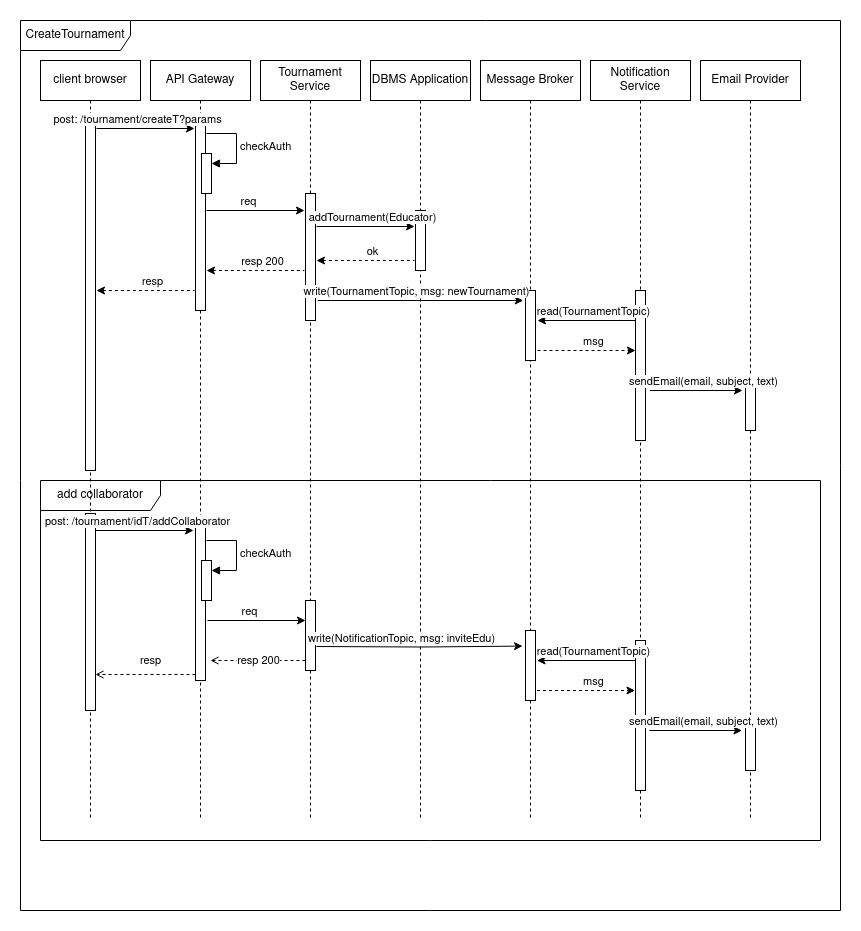
\includegraphics[width=1\linewidth]{misc//Images//UC/UC3.png}
    \caption{Create Tournament sequence diagram}
    \label{fig:enter-label}
\end{figure}
\newpage
\subsection{Subscribe To Tournament}

\begin{figure}[H]
    \centering
    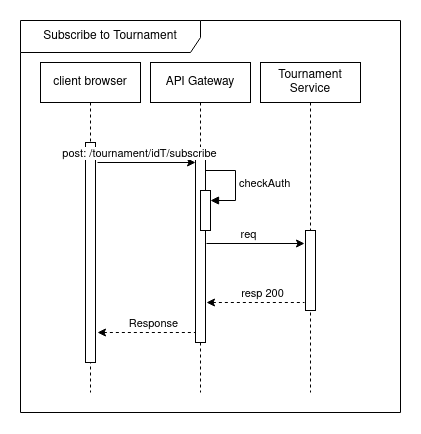
\includegraphics[width=1\linewidth]{misc//Images//UC/UC4.png}
    \caption{Subscribe To Tournament sequence diagram}
    \label{fig:enter-label}
\end{figure}
\newpage
\subsection{Create Battle}

At the end of the interaction the systems response contains the hyperlink to the newly created battle resource. An email is also sent to all the student users that are subscribed to the tournament, notifying them of the new available battle.

\begin{figure}[H]
    \centering
    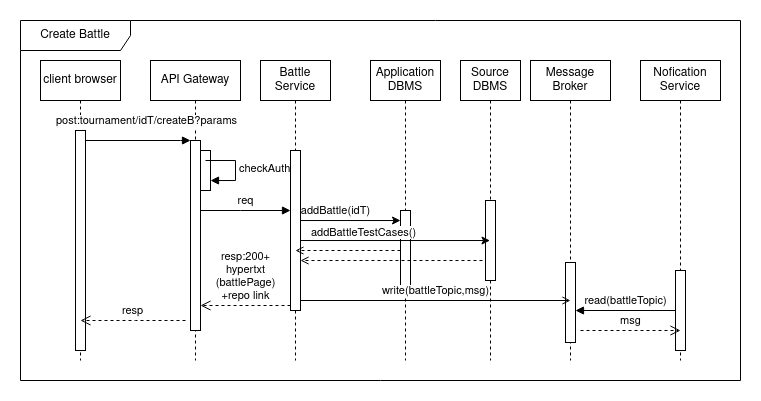
\includegraphics[width=1\linewidth]{misc//Images//UC/UC5.png}
    \caption{Create Battle sequence diagram}
    \label{fig:enter-label}
\end{figure}
\newpage
\subsection{Create Repository}

\begin{figure}[H]
    \centering
    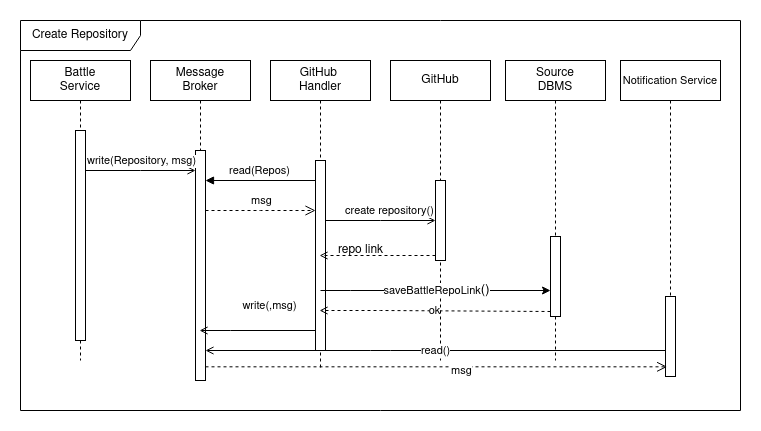
\includegraphics[width=1\linewidth]{misc//Images//UC/UC6.png}
    \caption{Create Repository sequence diagram}
    \label{fig:enter-label}
\end{figure}
\newpage
\subsection{Join Battle}

During the interaction the notification service sends an email the student listed from the user when joining the battle, notifying them of their position as group members in the battle.
If the battle group rules allows it and the user decide to join alone, the notification service won't read any message from the message broker, and no email will be sent.

\begin{figure}[H]
    \centering
    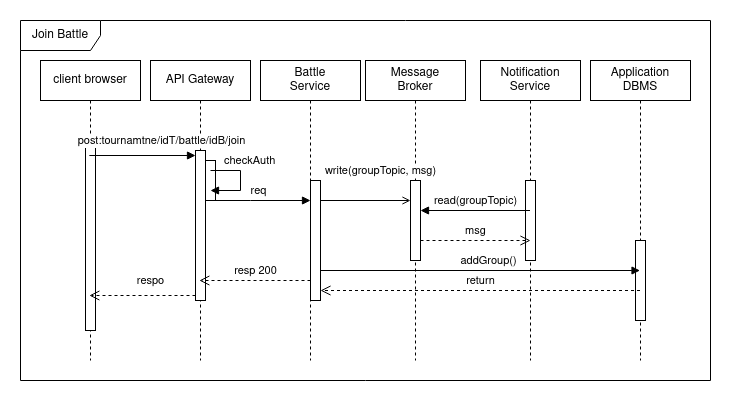
\includegraphics[width=1\linewidth]{misc//Images//UC/UC7.png}
    \caption{Join Battle sequence diagram}
    \label{fig:enter-label}
\end{figure}
\newpage
\subsection{Score Commit}

The interaction starts from GitHub notifying the system. Once the source code has been pulled it is stored in the source DBMS and a message notifying the new sources is sent to the message broker.
The software evaluation service is subscribed to the source topic and sees the notification, therefore it reads the sources from the source DBMS and starts to score the source code. Then it notifies the Leaderboard service with the new score through the message broker, which stores it as the group score in the application DBMS.

\begin{figure}[H]
    \centering
    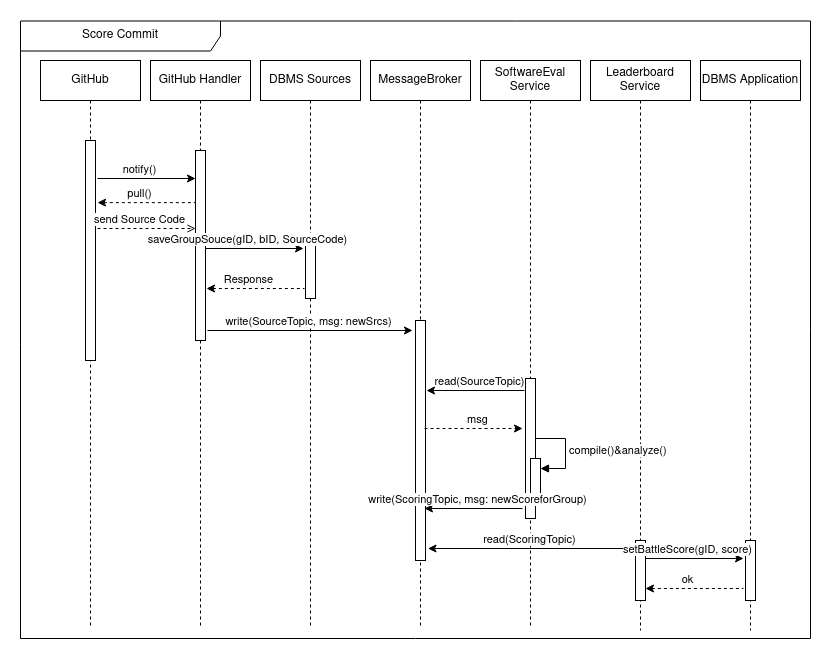
\includegraphics[width=1\linewidth]{misc//Images//UC/UC8.png}
    \caption{Score Commit sequence diagram}
    \label{fig:enter-label}
\end{figure}
\newpage
\subsection{View Battle Ranking}

The response received from the client contains the Battle Leaderboard data which will be visualized.

\begin{figure}[H]
    \centering
    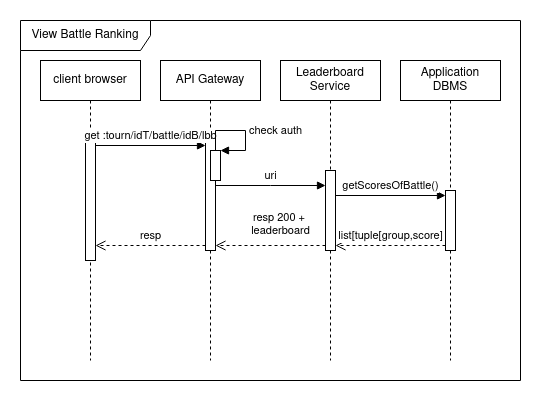
\includegraphics[width=1\linewidth]{misc//Images//UC/UC9.png}
    \caption{View Battle Ranking sequence diagram}
    \label{fig:enter-label}
\end{figure}
\newpage
\subsection{Manual Evaluation}

\begin{figure}[H]
    \centering
    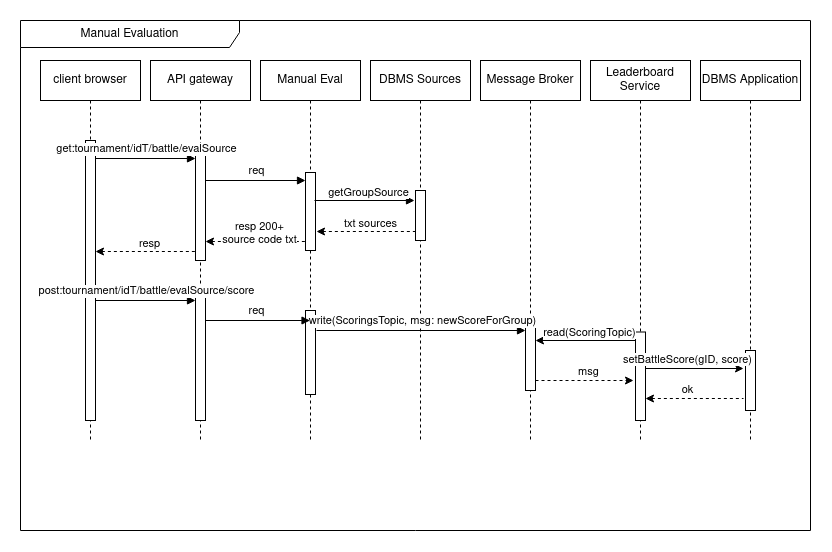
\includegraphics[width=1\linewidth]{misc//Images//UC/UC10.png}
    \caption{Manual Evaluation sequence diagram}
    \label{fig:enter-label}
\end{figure}
\newpage
\subsection{Look at Tournament Leaderboard}

The response received from the client contains the Tournament Leaderboard data which will be visualized.

\begin{figure}[H]
    \centering
    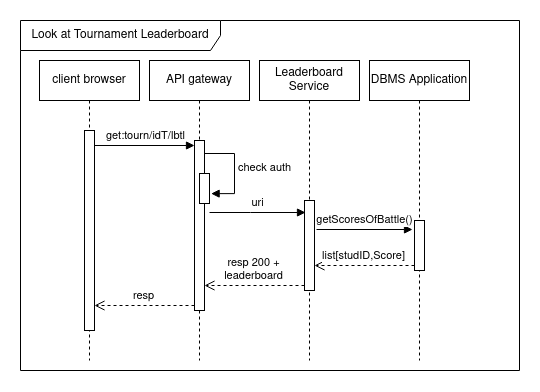
\includegraphics[width=1\linewidth]{misc//Images//UC/UC11.png}
    \caption{Look at Tournament Ranks sequence diagram}
    \label{fig:enter-label}
\end{figure}
\newpage
\subsection{Close Tournament}

\begin{figure}[H]
    \centering
    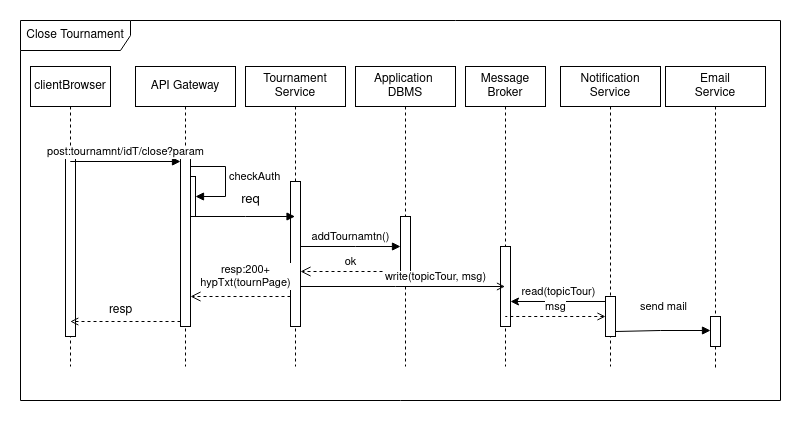
\includegraphics[width=1\linewidth]{misc//Images//UC/UC12.png}
    \caption{Close Tournament sequence diagram}
    \label{fig:enter-label}
\end{figure}
\newpage
\section{Component interfaces}

\subsection{Message Broker API}
The message broker exposes two methods:
\begin{itemize}
    \item read(Topic: int): Message: String
    \item write(Topic: int, Message: String)
\end{itemize}
All the microservices write/read on a particular topic exchanging JSON strings:



\begin{table}[h]
\hspace*{-4cm}
    \begin{tabular}{|c|c|c|c|}
    \hline
        \textbf{Topic} & \textbf{Publisher} & \textbf{Subscriber} & Content\\
    \hline
        Tournaments & Tournament Service & Notification Service & int: TournamentID, \\
         & & & bool: TournamentStatus \\
    \hline
        Battles & Battle Service & Notification Service & int BattleID,\\
        & & & int: BattleStatus \\
    \hline
        InvitationsBattle & Battle Service & Notification Service & int: groupID,\\
        & & & list[]: userID \\
    \hline
        InvitationsTournamet & Tournament Service & Notification Service & int: userID\\
        & & & int: TournamentID \\
    \hline
        Commits & GitHubHandler & SoftwareEval Service & int: groupID\\
    \hline
        Scores & ManualEval Service, SoftwareEval Service & Leaderboard Service & int: groupID\\
        & & & int: Score \\
    \hline
        Repository & Battle Service & GitHubHandler & int: battleID\\
    \hline
        RepoLinks & GithubHandler & Notification Service & int: battleID\\
        & & & String: LinkToRepository \\
    \hline
    \end{tabular}
    \hspace*{-4cm}
    \caption{Topics table}
    \label{tab:my_label}
\end{table}



\subsection{DBMS API}
\subsubsection{Data Access Interface}
Exposed by Application DBMS, used by Leaderboard, tournament, battle, group and user services. 
\begin{itemize}
    \item getSubscribedStudents(String : IDT): list[string studentID]
\end{itemize}
\paragraph{Used by Leaderboard Service}
\begin{itemize}
    \item getScoresOfTournament(String : IDT): Map[string: studenID; int: score]
    \item setScoresUserTournament(String:IDStud, String : IDT, int :score): void
    \item setScoresGroupBattle(String:IDGroup, String : IDB, int :score): void
    \item getScoresOfBattle(String: IDB): Map[ string: groupID, int: score]
\end{itemize}
\paragraph{Used by Notification Service}
\begin{itemize}
    \item getAllSignedStudent(): list[ string studID]
    \item getSubscribedStudent(string IDT): list[ string studID]
    \item getGroups(string IDB): map[string groupID; list[string studID]]
    \item getInvolvedEDUBattle(string IDB): list[ string eduID]
\end{itemize}
\paragraph{Used by Tournament Service}
\begin{itemize}
    \item addTournament(String : EduCreator):void
    \item grantBattleCreation(string : IDT, string : grantedEDU): void
    \item getCurrentTournamtn(): list[ string :tournamentID]
    \item getBattlesOfTourn(String : IDT):list[ string :battleID]
    \item checkEducatorPermission(String : IDT, String: IDEDU ): boolean response
\end{itemize}
\paragraph{Used by Battle Service}
\begin{itemize}
    \item getDeadlinesBattle(String: IDB): tuple(subsDL; submDL)
    \item addBattle(String TournamentID, string assignment,  int submDL, int subsDL, int maxsize, int minsize): string IDB
    \item getBattleAssignement(string IDB):  string assignment
    \item getBattleGroupRules(string IDB):  tuple(int  maxsize,int  minsize)
    \item getBattleAssignement(string IDB):  string assignment
    \item getBattleDeadlines(string IDB):  tuple(string submDL,string  subsDL)
    \item addGroup(list[string studID], String IDB): void
\end{itemize}
\paragraph{Used by User Service}
\begin{itemize}
    \item addStudent(String: UserName): void
    \item addEducator(String UserName): void
\end{itemize}
\subsubsection{Source Access Interface}
Exposed by Source DBMS, used by ManualEval, SoftwareEval, GithubHandler, Battle Service

\begin{itemize}
    \item addBattleTestCases(string IDB,list[ string] testcase):void
    \item getGroupSource(String: groupID, String: battleID): string SourceCodetxt
    \item saveGroupSource(String: groupID, String: battleID, String: SourceCodetxt): void
\end{itemize}
\subsection{RESTful API}
These are all external API's exposed by the API Gateway and used by the client application. They follow rest principle, each service handles some resources revolving around a particular aspect of the application i.e.: battles, tournaments, etc.  
Here follows a three of the uri path tree of the exposed resources:  
 
\begin{figure}[H]
    \centering
    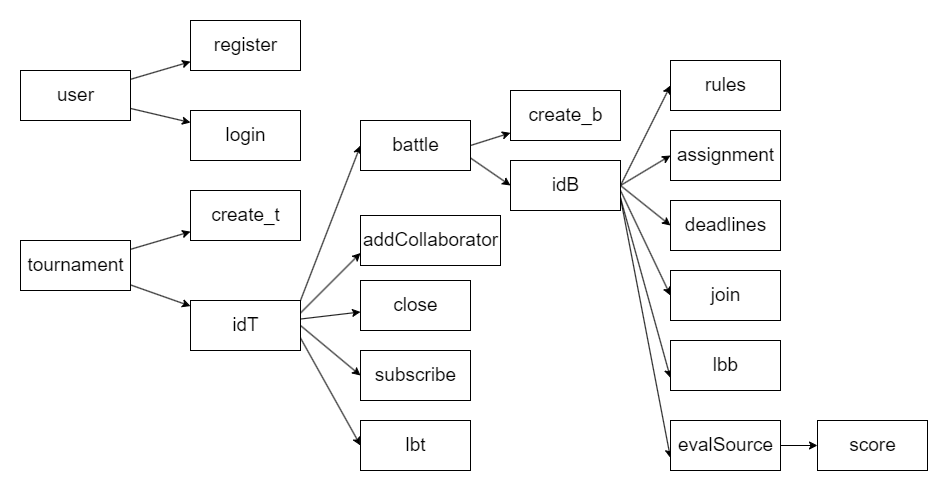
\includegraphics[width=1\linewidth]{misc//Images/RESTresources.png}
    \caption{Resource Tree path}
    \label{fig:enter-label}
\end{figure}
\subsubsection{UserAPI}

\begin{itemize}
\item \textbf{POST /user/register}\newline  
registerUser(StringU:UserName, String : UserType):void
\item \textbf{POST /user/login}\newline  
login(String : psw, String : UserID):void
\end{itemize}
\subsubsection{TournamentAPI}
\begin{itemize}
    \item \textbf{GET /tournament/}\newline  
    getCurrentTournament(String: UserId,String: UserType) : list$<$Tournament$>$
    \item \textbf{POST /tournament/create\_t}\newline  
    createTournament(String: UserId,String: UserType, String : TournamentName): void  
    \item \textbf{POST /tournament/{idT}/addCollaborator}\newline   
    addCollaborator(String: UserId,String: UserType, String : CollaboratorID):void  
    \item \textbf{POST /tournament/{idT}/close}\newline  
    closeTournament(String: UserId,String: UserType, String : TournamentID): void 
    \item  \textbf{POST /tournament/{idT}/subscribe}\newline  
    subscribeTournament(String: UserId,String: UserType, String : TournamentID) : void
    \item \textbf{GET /tournament/{idT}/battle/}\newline  
    getTournamentsBattles(String: UserId,String: UserType, String : TournamentID): List$<$Battle$>$  
\end{itemize}

\subsubsection{BattleAPI}
\begin{itemize}
    \item \textbf{POST /tournament/{idT}/battle/create\_b}\newline    
    createBattle(String: UserId,String: UserType, String : BattleName, tuple(int maxsize, int minsize): groupRule, string : assignemtent, tuple(date: subs, date: subm): deadline, list[ string]: testcases): void  
    \item \textbf{GET /tournament/{idT}/battle/{idB}/rules}\newline
     getGroupRules(String: UserId, String : BattleID): Tuple (int :MaxSize, int: MinSize)  
    \item \textbf{GET /tournament/{idT}/battle/{idB}/assignment}\newline  
     getAssignemntText(String: UserId, String : BattleId): String AssignmentText  
    \item \textbf{GET /tournament/{idT}/battle/{idB}/deadlines}\newline  
     getDeadlines(String: UserId, String : BattleID):Tuple (int :SubscriptionDL, int: SubmissionDL)  
    \item \textbf{POST /tournament/{idT}/battle/{idB}/join}\newline  
    joinBattle( String: UserId, String : BattleID, String: UserType, OPTIONAL List$<$ StudentID$>$ ): void
\end{itemize}

\subsubsection{LeaderBoardAPI}

\begin{itemize}
    \item \textbf{GET /tournament/{idT}/lbt}  \newline
    getLeaderBoardTournament(): LeaderBoard
    \item \textbf{GET /tournament/{idT}/battle/{idB}/lbb}  \newline
    getLeaderBoardBattle():Leaderboard  
\end{itemize}
\subsubsection{ManualEvaluationAPI}

\begin{itemize}
    \item \textbf{GET /tournament/{idT}/battle/evalSource}\newline
    getSourcesForEval(String: UserId, String : BattleID, String: UserType ): String SourceCode
    \item \textbf{POST /tournament/{idT}/battle/evalSource/score}\newline
    addManualScore(String: UserId, String : BattleID, String: UserType, int : score)
    : void
\end{itemize}
\section{Selected architectural styles and patterns}

\subsection{Microservices}

A microservice architecture is needed mainly in order to freely scale some component indipendently from others, like the \textbf{software evaluation} service, which at time may need much more computational resources, meanwhile other services are less likely to require as much, as they don't perform heavy activities like code analysis and execution.
Other then that, this style of architecture provides many more general advantages, making easy to choose. 

\subsubsection{API Gateway}

The API gateway provvides many benefits as the only entry point between the client and services.
Here are the ones which were more valued: Security and authentication; Load balancing; Caching. 

\subsection{Hybrid architecture (REST and EBA)}

\subsubsection{Event Based architecture}

Used in the system backend for the communication between microservices.  
The use of aynchronous communication allows for more flexibility and scalability, both important for some of the microservices, in particular the \textbf{software evaluation} service, which needs to scale indipndently from other services becaus of its higher computational needs.
Moreover the the system interfaces with Guthub APIs which have also an EBA.

\subsubsection{Rest(ful APIs)}

The services wich provide functionalities for the front end expose RESTful APIs.  
This way there is a greater separation of concern between front end and backend, as when developing the client application a team doesnt need to concern themeself with the internal structure of the system made of services, but only need to know the URI tree path used to access resources and their operations.

\section{Other design decisions}

There were no other design decisions to note.